\chapter{Pushdown Automata, CFG<-->PDA}

\section{CFG: Context Free Grammars}

Using FA and regular expressions, some language such as \(\{ 0^n1^n | n \geq 0 \} \) can not be described. 

\textbf{Context-free grammars}  is a more powerful method of describing languages. Such grammar can describe certain features that have a recursive structure, which makes them useful in a variety of applications.

An important application of CFG occurs in the specification and compilation of programming languages. A number of methodologies facilitate the construction of a \textbf{parser} once a CFG is available. Some tools even automatically generate the parser from the grammar.

\begin{example}[CFG example]
    The following CFG we call \(G_1\):

    \begin{align*}
        A &\rightarrow 0A1 \\
        A &\rightarrow B \\
        B &\rightarrow \# 
    \end{align*}

    Shorthand:
    \begin{align*}
        A &\rightarrow 0A1 | B \\
        B &\rightarrow \# 
    \end{align*}

    \begin{itemize}
        \item It contains a collection of \textbf{substitution rules}, also called \textbf{productions}. 
        \item Left side: \textbf{variable}, capital letters
        \item Right side: \textbf{terminals}, analogous to the input alphabet and often represented by lowercase letters, numbers or special symbols
        \item In this example, \(G_1\)'s variables are \(A\) and \(B\), its terminals are 0, 1 and \(\#\).   
    \end{itemize}

    Example of using \(G_1\) to generate string \verb|000#111|:
    \[
        A \Rightarrow 0A1 
        \Rightarrow 00A11
        \Rightarrow 000A111 
        \Rightarrow 000B111 
        \Rightarrow 000\#111 
    \] 

    The above information can be shown in a \textbf{parse tree}:

    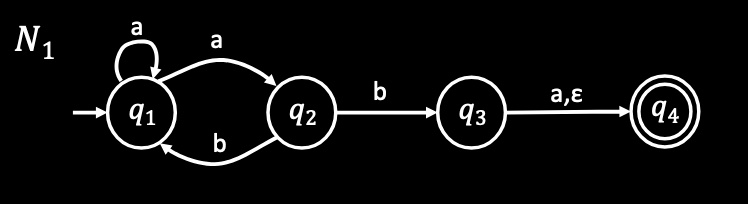
\includegraphics[width=0.8\textwidth]{f2.1.jpg}
\end{example}

\begin{definition}[CFG]
    A \textbf{context-free grammar} is a 4-tuple \((V, \Sigma, R, S)\), where
    \begin{enumerate}
        \item \(V\) is a finite set called the \textbf{variables}
        \item \(\Sigma\) is a finite set, disjoint from \(V\), called the \textbf{terminals}
        \item \(R\) is a finite set of \textbf{rules}, with each rule being a variable and a string of variables and terminals
        \item \(S \in V\) is the start variable       
    \end{enumerate}  
\end{definition}


